\chapter{Confronto tra amplificatori Nauta e Miller in termini di immunità EMI}
\label{chap:Nauta_Miller_Comparison}

Le architetture tradizionali degli amplificatori operazionali, come la configurazione Miller, hanno dimostrato una vulnerabilità alle EMI che può compromettere le prestazioni del sistema \cite{TR2016}. 

L'amplificatore Nauta, originariamente concepito come un transconduttore basato su inverter CMOS \cite{EMI_Immunity_of_the_Nauta_Inverter-Based_Amplifier}, rappresenta una potenziale alternativa alle architetture tradizionali per applicazioni che richiedono una maggiore robustezza alle EMI. La sua semplice topologia circuitale, priva di specchi di corrente e coppie differenziali, potrebbe offrire vantaggi significativi in termini di immunità alle interferenze.

Questo capitolo presenta un'analisi comparativa tra l'architettura Miller convenzionale e l'architettura Nauta, esaminando la loro rispettiva immunità ai disturbi elettromagnetici.

\section{Fondamenti Teorici della Suscettibilità EMI negli Amplificatori}

\subsection{Meccanismi di Suscettibilità EMI nelle Architetture Tradizionali}

La suscettibilità degli amplificatori operazionali alle EMI è principalmente dovuta a diversi fattori intrinseci alla loro architettura. Studi precedenti hanno identificato i seguenti fattori chiave:

\begin{itemize}
    \item \textbf{Asimmetria dello slew rate}: La differenza tra lo slew rate positivo e negativo genera una risposta non lineare quando il circuito è sottoposto a segnali EMI ad alta frequenza \cite{finalprint}.
    
    \item \textbf{Distorsione non lineare}: La presenza di coppie differenziali e specchi di corrente introduce non linearità che possono rettificare i segnali EMI, generando componenti DC indesiderate \cite{Redoute-Richelli_EMC_Magazine}.
    
    \item \textbf{Effetti capacitivi parassiti}: Le capacità parassite associate ai nodi interni possono facilitare l'accoppiamento dei segnali EMI all'interno del circuito \cite{An_EMI-Resistant_Common-Mode_Cancelation_Differential_Input_Stage_in_UMC_180_nm_CMOS}.
\end{itemize}

Nell'architettura Miller, questi fattori si manifestano principalmente attraverso la coppia differenziale d'ingresso e gli specchi di corrente costituenti il carico attivo. Quando un segnale EMI viene accoppiato agli ingressi dell'amplificatore, la coppia differenziale può generare un offset DC a causa della rettificazione non lineare del segnale interferente \cite{Design_considerations_for_an_ultra-low_voltage_amplifier_with_high_EMI_immunity}.

\begin{figure}[htbp]
    \centering
    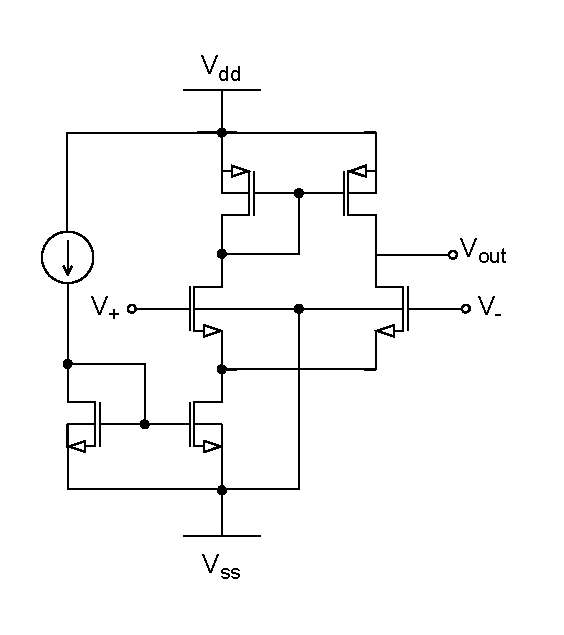
\includegraphics[width=0.8\textwidth]{img/sch/miller.drawio.pdf}
    \caption{Schema circuitale dell'architettura Miller.}
    \label{fig:miller_architecture}
\end{figure}

\subsection{Potenziali Vantaggi dell'Architettura Nauta}

L'architettura Nauta, di seguito mostrata nella figura \ref{fig:nauta_architecture}, presenta caratteristiche strutturali che potrebbero mitigare questi meccanismi di suscettibilità:

\begin{itemize}
    \item \textbf{Assenza di coppie differenziali}: L'utilizzo di inverter CMOS come elemento base elimina la necessità di coppie differenziali tradizionali.
    
    \item \textbf{Simmetria intrinseca}: Gli inverter CMOS offrono naturalmente una risposta più simmetrica, con slew rate positivo e negativo potenzialmente più bilanciati \cite{EMI_Immunity_of_the_Nauta_Inverter-Based_Amplifier}.
    
    \item \textbf{Topologia semplificata}: L'assenza di nodi interni riduce il numero di punti vulnerabili all'accoppiamento EMI.
    
    \item \textbf{Comportamento lineare in regione di forte inversione}: Quando i transistor operano in forte inversione, l'amplificatore Nauta offre una buona linearità nella conversione tensione-corrente.
\end{itemize}

% Qui si potrebbe inserire una figura che confronta le topologie di base di un amplificatore Miller e di un amplificatore Nauta, evidenziando le differenze strutturali

\begin{figure}[H]
    \begin{subfigure}{0.66\textwidth}
        \centering
        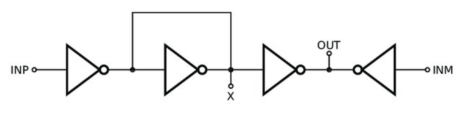
\includegraphics[width=0.8\textwidth]{img/nauta-ota-single-ended.pdf}
        \caption{Schema circuitale dell'amplificatore Nauta.}
        \label{fig:nauta_single_ended}        
    \end{subfigure}    
    \hfill
    \begin{subfigure}{0.33\textwidth}
        \centering
        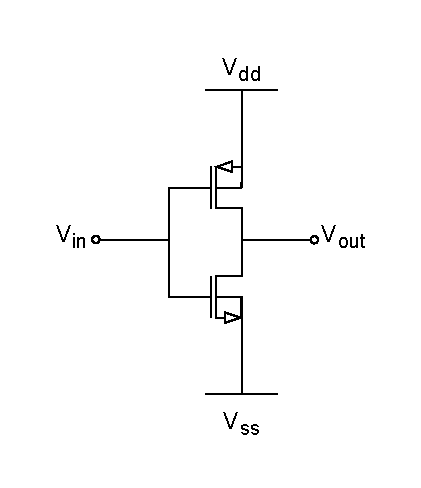
\includegraphics[width=0.8\textwidth]{img/sch/inverter.drawio.pdf}
        \caption{Schema circuitale dell'inverter CMOS.}
        \label{fig:nauta_inverter}
    \end{subfigure}
    \caption{Schema circuitale dell'architettura Nauta.}
    \label{fig:nauta_architecture}
\end{figure}

\section{Metodologia di Simulazione}

Per valutare comparativamente l'immunità alle EMI delle architetture Miller e Nauta, è stato sviluppato un approccio di simulazione sistematico utilizzando il simulatore Cadence Virtuoso \textcopyright. L'obiettivo è quantificare e confrontare la risposta di entrambe le architetture quando sottoposte a disturbi elettromagnetici in diverse configurazioni.

\subsection{Setup di Simulazione}

Le simulazioni sono state configurate secondo le seguenti specifiche:

\begin{itemize}
    \item \textbf{Configurazione circuitale}: Entrambi gli amplificatori sono stati configurati come inseguitori di tensione (voltage followers). \todo{aggiungere spiegaizone sulla scelta della configurazione?}
    
    \item \textbf{Modellazione EMI}: I disturbi elettromagnetici sono stati modellati come segnali sinusoidali accoppiati ai terminali degli amplificatori, con frequenze variabili da 1 MHz a 3-4 GHz.
    
    \item \textbf{Punti di iniezione EMI}: Sono stati considerati come punti di iniezione del disturbo solo i terminali di ingresso degli amplificatori.
    
    \item \textbf{Parametri di valutazione}: Per ogni configurazione, sono stati misurati lo spostamento del punto di lavoro DC (offset).
\end{itemize}

\subsection{Varianti Architetturali Analizzate}

Lo studio ha incluso la simulazione delle seguenti varianti:

\begin{itemize}
    \item \textbf{Amplificatore Miller a singolo stadio}: Implementazione tradizionale con coppia differenziale e carico attivo.
    \begin{figure}[H]
        \centering
        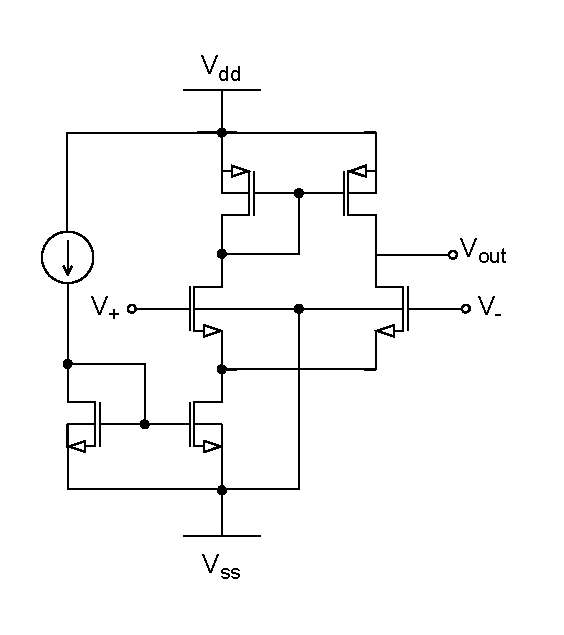
\includegraphics[width=0.4\textwidth]{img/sch/miller.drawio.pdf}
        \caption{Schema circuitale dell'amplificatore Miller a singolo stadio.}
        \label{fig:miller_single_stage}
    \end{figure}
    
    \item \textbf{Amplificatore Miller a due stadi}: Configurazione mille con stadio aggiuntivo e rete di compensazione \textit{R-C} per migliorare la stabilità e il guadagno.
    \begin{figure}[H]
        \centering
        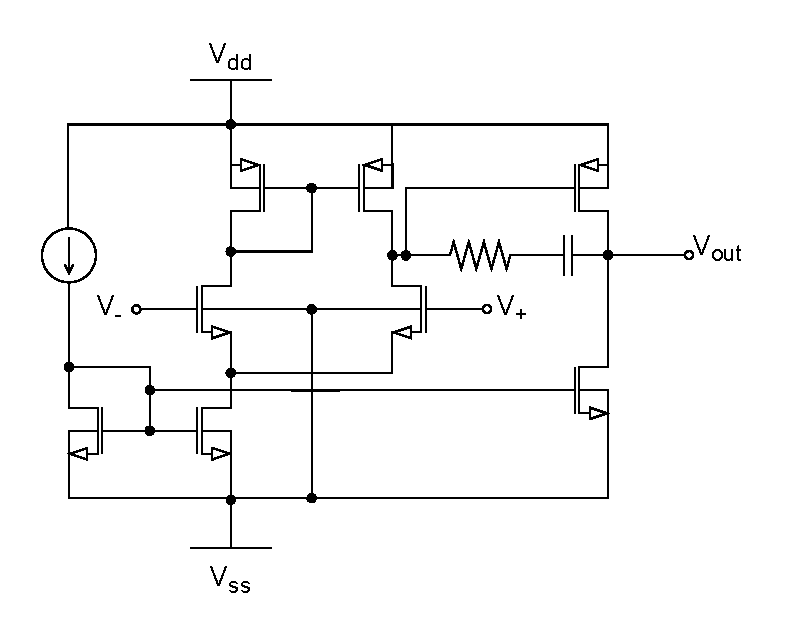
\includegraphics[width=0.5\textwidth]{img/sch/miller_two_staged.drawio.pdf}
        \caption{Schema circuitale dell'amplificatore Miller a due stadi.}
        \label{fig:miller_double_stage}
    \end{figure}
    
    \item \textbf{Amplificatore Nauta a singolo stadio}: Implementazione inverter-based seguendo la topologia originale proposta da Nauta.
    \begin{figure}[H]
        \centering
        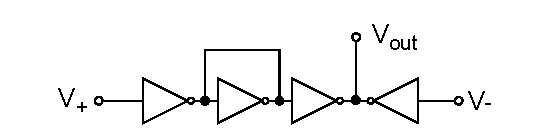
\includegraphics[width=0.6\textwidth]{img/sch/basic_nauta.pdf}
        \caption{Schema circuitale dell'amplificatore Nauta a singolo stadio.}
        \label{fig:nauta_single_stage}
    \end{figure}
    
    \item \textbf{Amplificatore Nauta a due stadi}: Versione modificata con due stadi in cascata per aumentare il guadagno.
    \begin{figure}[H]
        \centering
        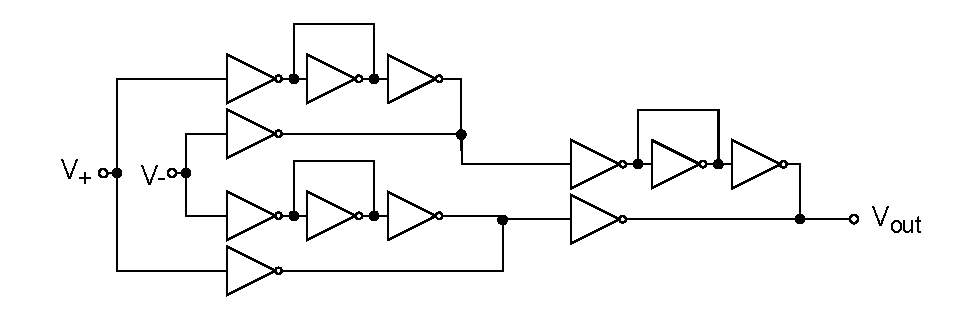
\includegraphics[width=0.8\textwidth]{img/sch/nauta_two_staged.pdf}
        \caption{Schema circuitale dell'amplificatore Nauta a due stadi.}
        \label{fig:nauta_double_stage}
    \end{figure}
\end{itemize}

% Qui si potrebbe inserire una figura che mostra gli schematici dettagliati delle quattro varianti implementate

\subsection{Parametri di Confronto}

Per garantire un confronto equo, i circuiti sono stati progettati per avere specifiche comparabili in termini di:

\begin{itemize}
    \item Guadagno a circuito aperto: circa 40 dB per gli amplificatori a singolo stadio.
    \item Prodotto guadagno-banda (GBWP): circa 1-2MHz.
    \item Margine di fase (almeno 60 gradi).
    \item CMRR: almeno 60 dB.
\end{itemize}

Si sono valutate le configurazioni con carico capacitivo di 1pF e 10pF per simulare la variazione delle prestazioni al variare degli effetti parassiti.
\section{Importanza di un elevato CMRR nella mitigazione delle EMI}

I sistemi elettronici moderni operano in ambienti elettromagneticamente rumorosi, dove i segnali EMI si accoppiano principalmente in modo comune ai due ingressi degli amplificatori differenziali. Come evidenziato in \cite{finalprint}, una delle principali sfide nei sistemi di acquisizione è che i cavi di interconnessione tra sensori e circuiti di condizionamento agiscono come antenne indesiderate per le EMI irradiate.

Il CMRR, definito come il rapporto tra il guadagno differenziale e il guadagno di modo comune ($CMRR = \frac{A_{dm}}{A_{cm}}$), quantifica la capacità di un amplificatore di rigettare i segnali che appaiono identicamente su entrambi gli ingressi. L'importanza di un alto CMRR nella mitigazione delle EMI deriva da diversi fattori:

\begin{enumerate}
    \item \textbf{Prevalenza di EMI di modo comune}: Come spiegato in \cite{finalprint}, le EMI si accoppiano principalmente come segnali di modo comune poiché i cavi di interconnessione sono instradati vicini tra loro. Questi segnali EMI possono raggiungere ampiezze nell'ordine di decine di volt, mentre i segnali differenziali utili dei sensori sono spesso nell'ordine dei millivolt.
    
    \item \textbf{Conversione modo comune-differenziale}: Secondo \cite{An_EMI-Resistant_Common-Mode_Cancelation_Differential_Input_Stage_in_UMC_180_nm_CMOS}, quando un amplificatore è esposto simultaneamente a segnali EMI di modo comune e differenziale, si genera una tensione di offset DC. L'espressione di questa tensione di offset è:
    
    \[V_{OS} = \frac{1}{V_{GS} - V_{th}} \int_{-\infty}^{+\infty} |H_c(j\omega) \cdot V_c(j\omega) \cdot V_d(j\omega)| \cdot \cos\phi \cdot d\omega\]
    
    dove $H_c(j\omega)$ è la funzione di trasferimento per i segnali di modo comune. Un alto CMRR riduce $H_c(j\omega)$, diminuendo così l'offset indotto.
    
    \item \textbf{Capacità parassite}: Come evidenziato in \cite{Redoute-Richelli_EMC_Magazine}, la capacità parassita alla sorgente della coppia differenziale ($C_T$) aumenta la funzione di trasferimento di modo comune alle alte frequenze EMI, contribuendo alla generazione di offset. Un alto CMRR aiuta a compensare questo effetto.
    
    \item \textbf{Prevenzione della saturazione}: Nel caso di EMI di grande ampiezza, un insufficiente CMRR può causare la saturazione dell'amplificatore, compromettendo completamente il suo funzionamento, come mostrato in \cite{TR2016}.
\end{enumerate}
\todo{Rivedere le citazioni inserite e le formule riportate.}
Le architetture di amplificatori con CMRR elevato, come quelle che utilizzano tecniche di cancellazione del modo comune \cite{An_EMI-Resistant_Common-Mode_Cancelation_Differential_Input_Stage_in_UMC_180_nm_CMOS} o coppie differenziali completamente simmetriche \cite{EMI_Immunity_of_the_Nauta_Inverter-Based_Amplifier}, sono quindi essenziali in ambienti elettromagneticamente ostili. Queste architetture possono ridurre l'offset indotto dalle EMI di un ordine di grandezza rispetto alle topologie convenzionali.

\section{Testo aggiuntivo scartato}
\subsection{Considerazioni Preliminari sull'Immunità EMI}

Sulla base dell'analisi teorica e delle simulazioni preliminari, sono state formulate le seguenti ipotesi riguardo alle prestazioni di immunità EMI delle due architetture:

\subsubsection{Vantaggi Previsti dell'Architettura Nauta}

\begin{itemize}
    \item \textbf{Maggiore simmetria intrinseca}: La struttura basata su inverter dovrebbe garantire una risposta più simmetrica ai disturbi, riducendo la rettificazione non lineare.
    
    \item \textbf{Minore sensibilità alla frequenza EMI}: L'assenza di nodi interni potrebbe ridurre la variazione della suscettibilità in funzione della frequenza.
    
    \item \textbf{Migliore comportamento agli estremi della banda}: La risposta più simmetrica dovrebbe mitigare i picchi di suscettibilità alle alte frequenze.
\end{itemize}

\subsubsection{Sfide Potenziali dell'Architettura Nauta}

\begin{itemize}
    \item \textbf{Limitazioni di guadagno}: Il guadagno intrinsecamente limitato potrebbe richiedere stadi aggiuntivi, introducendo potenziali vulnerabilità.
    
    \item \textbf{Sensibilità alle variazioni di processo}: La dipendenza da un preciso bilanciamento PMOS/NMOS potrebbe rendere le prestazioni più sensibili alle variazioni di processo.
    
    \item \textbf{Consumo di potenza}: L'implementazione classica potrebbe richiedere un maggiore consumo di potenza rispetto ad alcune varianti dell'architettura Miller.
\end{itemize}

\subsection{Conclusioni}

Questo capitolo ha presentato il framework metodologico per la valutazione comparativa dell'immunità EMI degli amplificatori basati sulle architetture Miller e Nauta. L'approccio sistematico sviluppato permette di quantificare obiettivamente le prestazioni in presenza di disturbi elettromagnetici, considerando diversi punti di iniezione, frequenze e ampiezze.

La semplice topologia circuitale dell'amplificatore Nauta, priva di specchi di corrente e coppie differenziali, offre potenzialmente vantaggi significativi in termini di immunità EMI. Le simulazioni dettagliate e i risultati quantitativi di questo confronto saranno presentati e discussi nel capitolo successivo, fornendo indicazioni concrete sulla superiorità relativa di ciascuna architettura in diversi scenari applicativi.

% Riferimenti bibliografici verranno gestiti automaticamente dal sistema BibTeX

\subsection{Fondamenti teorici dell'analisi EMI}

\subsubsection{Formula dell'offset di tensione indotto dalle EMI}

Secondo Redouté e Richelli \cite{Redoute-Richelli_EMC_Magazine}, l'offset di tensione indotto dalle EMI può essere espresso dalla seguente formula:

\begin{equation}
V_{OS} = \frac{1}{V_{GS} - V_{th}} \int_{-\infty}^{+\infty} |H_c(j\omega) \cdot V_c(j\omega) \cdot V_d(j\omega)| \cdot \cos\phi \cdot d\omega
\end{equation}

dove:
\begin{equation}
\phi = \arctan\left(\frac{\text{Im}\{H_c(j\omega) \cdot V_c(j\omega) \cdot V_d(j\omega)\}}{\text{Re}\{H_c(j\omega) \cdot V_c(j\omega) \cdot V_d(j\omega)\}}\right)
\end{equation}

e $H_c(j\omega)$ è la funzione di trasferimento per i segnali di modo comune, $V_{GS}$ è la tensione gate-source di polarizzazione, e $V_{th}$ è la tensione di soglia. Questa formula evidenzia che l'offset indotto dalle EMI dipende dalla funzione di trasferimento di modo comune, dall'ampiezza delle componenti di modo comune e differenziale, e dalla fase tra queste componenti.

\subsubsection{Specificazione dei metodi di test e validazione}

Per quanto riguarda la metodologia di analisi, Richelli et al. \cite{TR2016} descrivono la configurazione sperimentale standard:

\begin{quote}
``Per verificare il grado di immunità alle interferenze elettromagnetiche del dispositivo sono state eseguite delle simulazioni in cui si è utilizzato l'amplificatore in configurazione a inseguitore di tensione, a questo si è fornito in ingresso un segnale sinusoidale e si è rilevato il valore dell'offset di uscita al variare della frequenza iniettata.''
\end{quote}

\subsubsection{Validità dei risultati - livelli di segnale}

Riguardo alle soglie minime per considerare validi i risultati, Zuccarotto \cite{tesi} osserva nell'analisi degli specchi di corrente:

\begin{quote}
``Per rendere lo specchio di corrente più robusto alle interferenze, senza modificarne la topologia, è consigliabile avere una corrente $I_{DC}$ che non sia confrontabile con la $i_{EMI}$.''
\end{quote}

Richelli et al. \cite{TR2016} forniscono questa importante osservazione sulla relazione tra livelli di segnale e validità dei risultati:

\begin{quote}
``EMI coupling at the power supply and input pins is weak (the voltage generators have a small internal resistance and we can consider $R_{par} = 50\Omega$ as the worst case). Conversely, the coupling is very pronounced at the output pin which is a higher impedance node.''
\end{quote}

\subsubsection{Modellazione degli effetti parassiti}

Per modellare correttamente gli effetti parassiti che influenzano le prestazioni EMI, Zuccarotto \cite{tesi} utilizza:

\begin{equation}
C_{eq} \simeq C_{db2a} + C_{db4a}
\end{equation}

Dove la capacità parassita $C_{db}$ è dovuta alla giunzione drain-bulk polarizzata inversamente e descritta dalla formula:

\begin{equation}
C_j = \sqrt{\frac{q\epsilon_s N_B}{2(V_{bi} - V)}}
\end{equation}

Questa formula, estratta da \cite{tesi}, mostra come la capacità di svuotamento vari con la tensione applicata alla giunzione, influenzando così la risposta alle EMI.

\subsubsection{Caratterizzazione della suscettibilità alle EMI}

Per la caratterizzazione della suscettibilità alle EMI, Richelli et al. \cite{Measurements_of_EMI_susceptibility_of_precision_voltage_references} specificano:

\begin{quote}
``Il parametro utilizzato per valutare la suscettibilità alle EMI è la tensione di offset in uscita, misurata come lo scostamento del valore medio della tensione di uscita rispetto al valore nominale.''
\end{quote}

\subsubsection{Asimmetria dello slew rate}

Riguardo all'asimmetria dello slew rate come causa di suscettibilità alle EMI, Zuccarotto \cite{tesi} osserva:

\begin{quote}
``L'asimmetria deriva dal fatto che le correnti di carica e scarica non sono necessariamente uguali, infatti nei diversi transistor gli effetti parassiti modificano tale valore. Tale limitazione diventa determinante al crescere della frequenza.''
\end{quote}

E aggiunge la formula che lega lo slew rate alla frequenza massima del segnale:

\begin{equation}
\max\left(\frac{dV_i(t)}{dt}\right) = \omega A
\end{equation}

\begin{quote}
``Finché $\omega A \leq SR$ l'uscita segue l'ingresso senza problemi. Superata tale soglia, però, l'uscita risulta essere sempre più distorta rispetto al segnale d'ingresso.''
\end{quote}